\section{Конструкторская часть}

В данном разделе описаны сущности системы, приведена диаграмма БД, описана проектируемая функция базы данных и приведена формализация бизнес-правил разрабатываемого приложения.

\subsection{Описание сущностей}

На основе выделенных ранее сущностей спроектированны таблицы реляционной базы данных.

\subsubsection{Таблица users}

Эта таблица содержит информацию о пользователях системы и включает поля:

\begin{enumerate}[label=\arabic*.]
    \item uuid --- идентификатор, тип --- uuid, является первичным ключем;
    \item created\_at --- временная метка создания, тип --- timestamp;
    \item updated\_at --- временная метка обновления, тип --- timestamp;
    \item deleted\_at --- временная метка удаления, тип --- timestamp. Будет null, если запись не является удаленной;
    \item phone --- телефон, тип text, уникальное;
    \item login --- логин, тип text, уникальное;
    \item password\_hash --- хэш пароля, тип text;
    \item role --- роль, тип text;
\end{enumerate}

\subsubsection{Таблица tags}

Эта таблица содержит информацию о тегах и включает поля:

\begin{enumerate}[label=\arabic*.]
	\item uuid --- идентификатор, тип --- uuid, является первичным ключем;
	\item created\_at --- временная метка создания, тип --- timestamp;
	\item updated\_at --- временная метка обновления, тип --- timestamp;
	\item deleted\_at --- временная метка удаления, тип --- timestamp. Будет null, если запись не является удаленной;
	\item name --- название, тип text, уникальное;
	\item description --- описание, тип text;
\end{enumerate}

\subsubsection{Таблица events}

Эта таблица содержит информацию о событиях и включает поля:

\begin{enumerate}[label=\arabic*.]
	\item uuid --- идентификатор, тип --- uuid, является первичным ключем;
	\item created\_at --- временная метка создания, тип --- timestamp;
	\item updated\_at --- временная метка обновления, тип --- timestamp;
	\item deleted\_at --- временная метка удаления, тип --- timestamp. Будет null, если запись не является удаленной;
	\item timestamp --- временная метка события, тип --- timestamp;
	\item name --- название, тип text;
	\item description --- описание, тип text;
	\item type --- тип события, тип text;
	\item is\_whole\_day --- признак, что событие занимает целый день, тип bool;
	\item creator\_uuid --- ссылка на создателя события, тип uuid;
\end{enumerate}

\subsubsection{Таблица events\_tags}

Эта таблица-связка событий и тегов. Включает поля:

\begin{enumerate}[label=\arabic*.]
	\item event\_uuid --- ссылка на событие, тип uuid;
	\item tag\_uuid --- ссылка на тег, тип uuid;
\end{enumerate}

\subsubsection{Таблица access\_rights}

Эта таблица содержит информацию о правах доступа и включает поля:

\begin{enumerate}[label=\arabic*.]
	\item code --- название, тип text, является первичным ключем;
	\item description --- описание, тип text;
\end{enumerate}

\subsubsection{Таблица invitations}

Эта таблица содержит информацию о приглашениях и включает поля:

\begin{enumerate}[label=\arabic*.]
	\item uuid --- идентификатор, тип --- uuid, является первичным ключем;
	\item access\_right\_code --- ссылка на код права доступа, тип text;
	\item event\_uuid --- ссылка на событие, тип uuid;
	\item user\_uuid --- ссылка на приглашенного пользователя, тип uuid;
\end{enumerate}

\subsubsection{Схема базы данных}

На рисунке \ref{fig:DB} представлена диаграмма базы данных.

\begin{figure}[ht!]
	\centering
	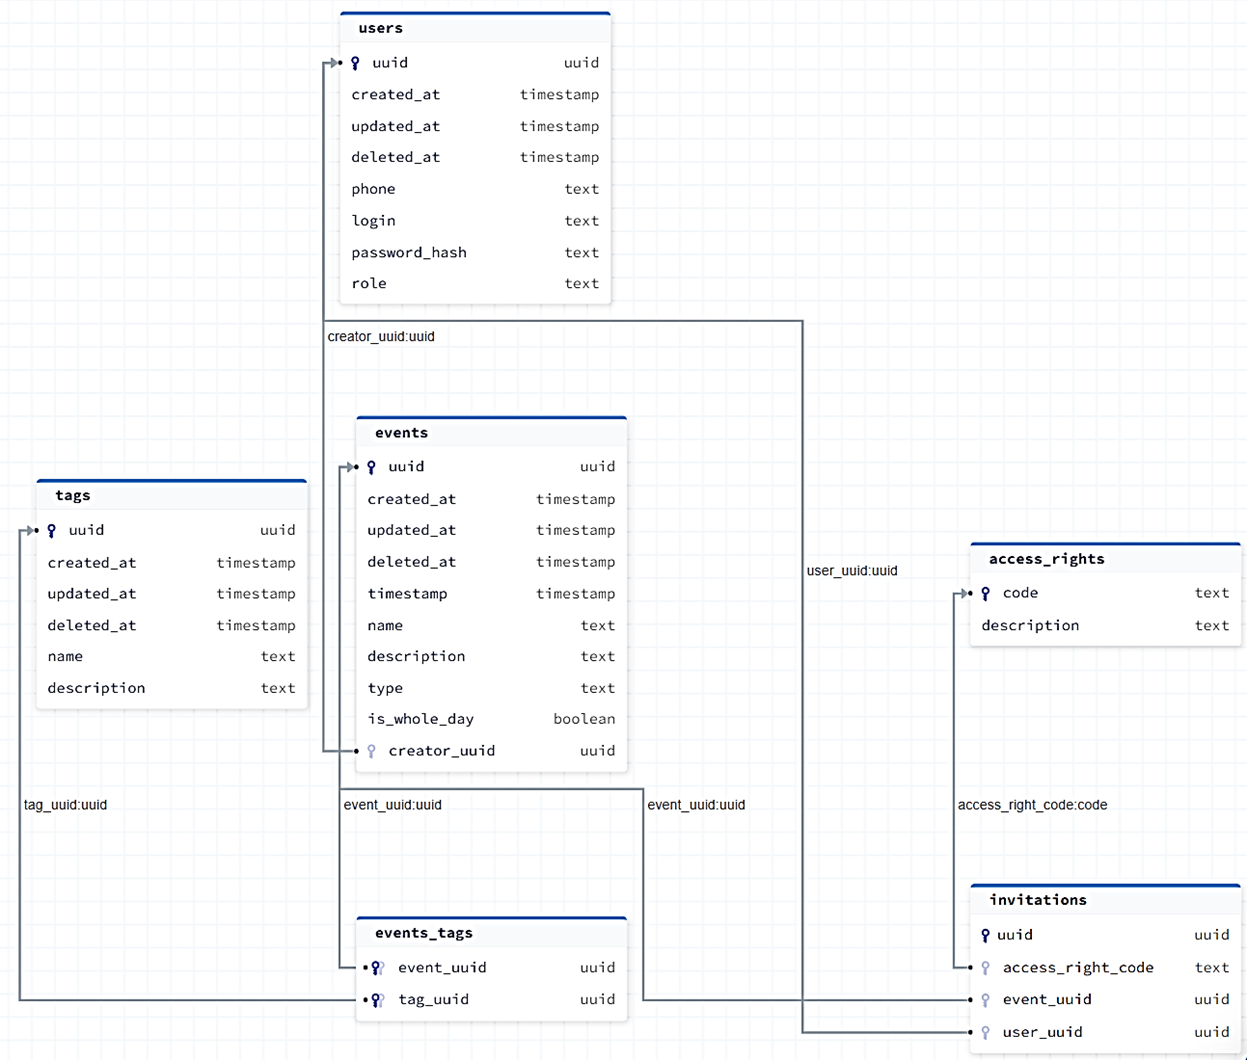
\includegraphics[width=0.9\linewidth]{assets/images/DB.png}
	\caption{Схема базы данных Postgres}
	\label{fig:DB}
\end{figure}
\FloatBarrier

\subsubsection{Схема индекса ElasticSearch}

На листинге \ref{lst:ES} представлено описание схемы индекса events в ElasticSearch.

\begin{center}
	\captionsetup{justification=raggedright,singlelinecheck=off}
	\begin{lstlisting}[label=lst:ES,caption=Схема индекса events]
"mappings": {
	"properties": {
		"@indexed_at": {
			"type": "date"
		},
		"Creator": {
			"properties": {
				"Login": {
					"type": "text",
					"fields": {
						"keyword": {
							"type": "keyword",
							"ignore_above": 256
						}
					}
				},
				"PasswordHash": {
					"type": "text",
					"fields": {
						"keyword": {
							"type": "keyword",
							"ignore_above": 256
						}
					}
				},
				"Phone": {
					"type": "text",
					"fields": {
						"keyword": {
							"type": "keyword",
							"ignore_above": 256
						}
					}
				},
				"Role": {
					"type": "text",
					"fields": {
						"keyword": {
							"type": "keyword",
							"ignore_above": 256
						}
					}
				},
				"Uuid": {
					"type": "text",
					"fields": {
						"keyword": {
							"type": "keyword",
							"ignore_above": 256
						}
					}
				}
			}
		},
		"CreatorUuid": {
			"type": "text",
			"fields": {
				"keyword": {
					"type": "keyword",
					"ignore_above": 256
				}
			}
		},
		"Description": {
			"type": "text",
			"fields": {
				"keyword": {
					"type": "keyword",
					"ignore_above": 256
				}
			}
		},
		"Invitations": {
			"properties": {
				"AccessRightCode": {
					"type": "text",
					"fields": {
						"keyword": {
							"type": "keyword",
							"ignore_above": 256
						}
					}
				},
				"UserUuid": {
					"type": "text",
					"fields": {
						"keyword": {
							"type": "keyword",
							"ignore_above": 256
						}
					}
				},
				"Uuid": {
					"type": "text",
					"fields": {
						"keyword": {
							"type": "keyword",
							"ignore_above": 256
						}
					}
				}
			}
		},
		"IsWholeDay": {
			"type": "boolean"
		},
		"Name": {
			"type": "text",
			"fields": {
				"keyword": {
					"type": "keyword",
					"ignore_above": 256
				}
			}
		},
		"Tags": {
			"properties": {
				"Description": {
					"type": "text",
					"fields": {
						"keyword": {
							"type": "keyword",
							"ignore_above": 256
						}
					}
				},
				"Name": {
					"type": "text",
					"fields": {
						"keyword": {
							"type": "keyword",
							"ignore_above": 256
						}
					}
				},
				"Uuid": {
					"type": "text",
					"fields": {
						"keyword": {
							"type": "keyword",
							"ignore_above": 256
						}
					}
				}
			}
		},
		"Timestamp": {
			"type": "date"
		},
		"Type": {
			"type": "text",
			"fields": {
				"keyword": {
					"type": "keyword",
					"ignore_above": 256
				}
			}
		},
		"Uuid": {
			"type": "text",
			"fields": {
				"keyword": {
					"type": "keyword",
					"ignore_above": 256
				}
			}
		}
	}
},
	\end{lstlisting}
\end{center}
  

\subsection{Описание проектируемой процедуры}
Для корректной работы ролевой системы перед каждым запросом требуется устанавливать необходимую роль текущему пользователю и заносить его \textit{uuid} в переменную текущего сеанса \textbf{app.user\_uuid}. 

Для выполнения описанных выше действий была спроектирована хранимая процедура. Схема ее алгоритма представлена на рисунке \ref{fig:DB-func}.

\begin{figure}[ht!]
	\centering
	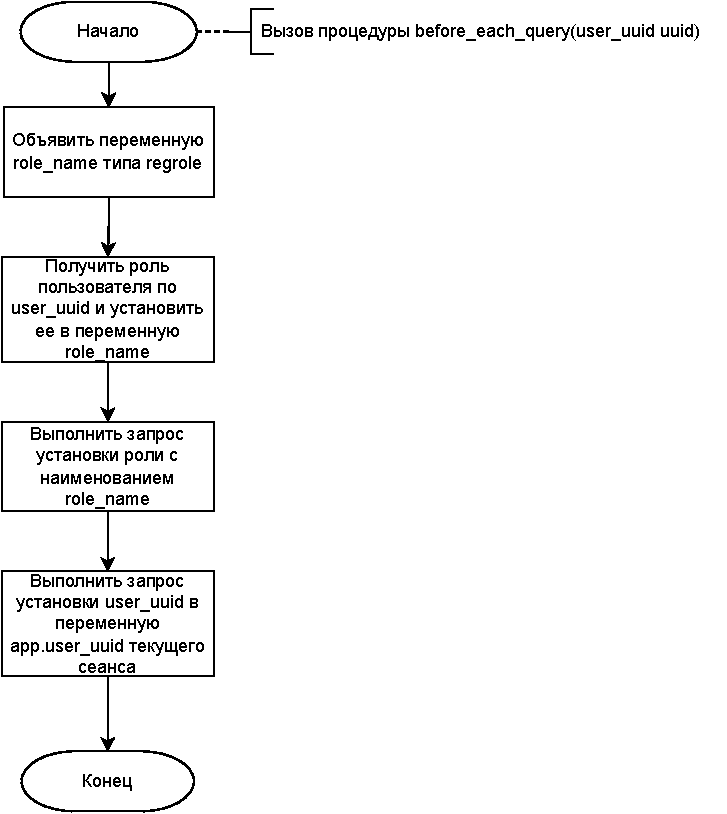
\includegraphics[width=0.9\linewidth]{assets/images/Func.pdf}
	\caption{Функция для установки роли и uuid-а текущего пользователя}
	\label{fig:DB-func}
\end{figure}

\subsection{Проектирование приложения}

В рамках поставленной задачи курсового проекта необходимо разработать веб-приложение с программным интерфейсой (API), обрабатывающим запросы согласно спецификации GraphQL \cite{graphql-spec}. API должен позволять пользователям выполнять в системе действия, представленные на диаграмме вариантов использования (рисунки \ref{fig:use-case-simple} -- \ref{fig:use-case-admin}).

Незарегистрированный пользователь должен иметь возможность создать новый аккаунт или войти в уже существующий аккаунт. Формализация бизнес-процессов авторизации и регистрации в нотации Business Process Model and Notation (BPMN) представлена на рисунке \ref{fig:BPMN-auth}.

\begin{figure}[ht!]
	\centering
	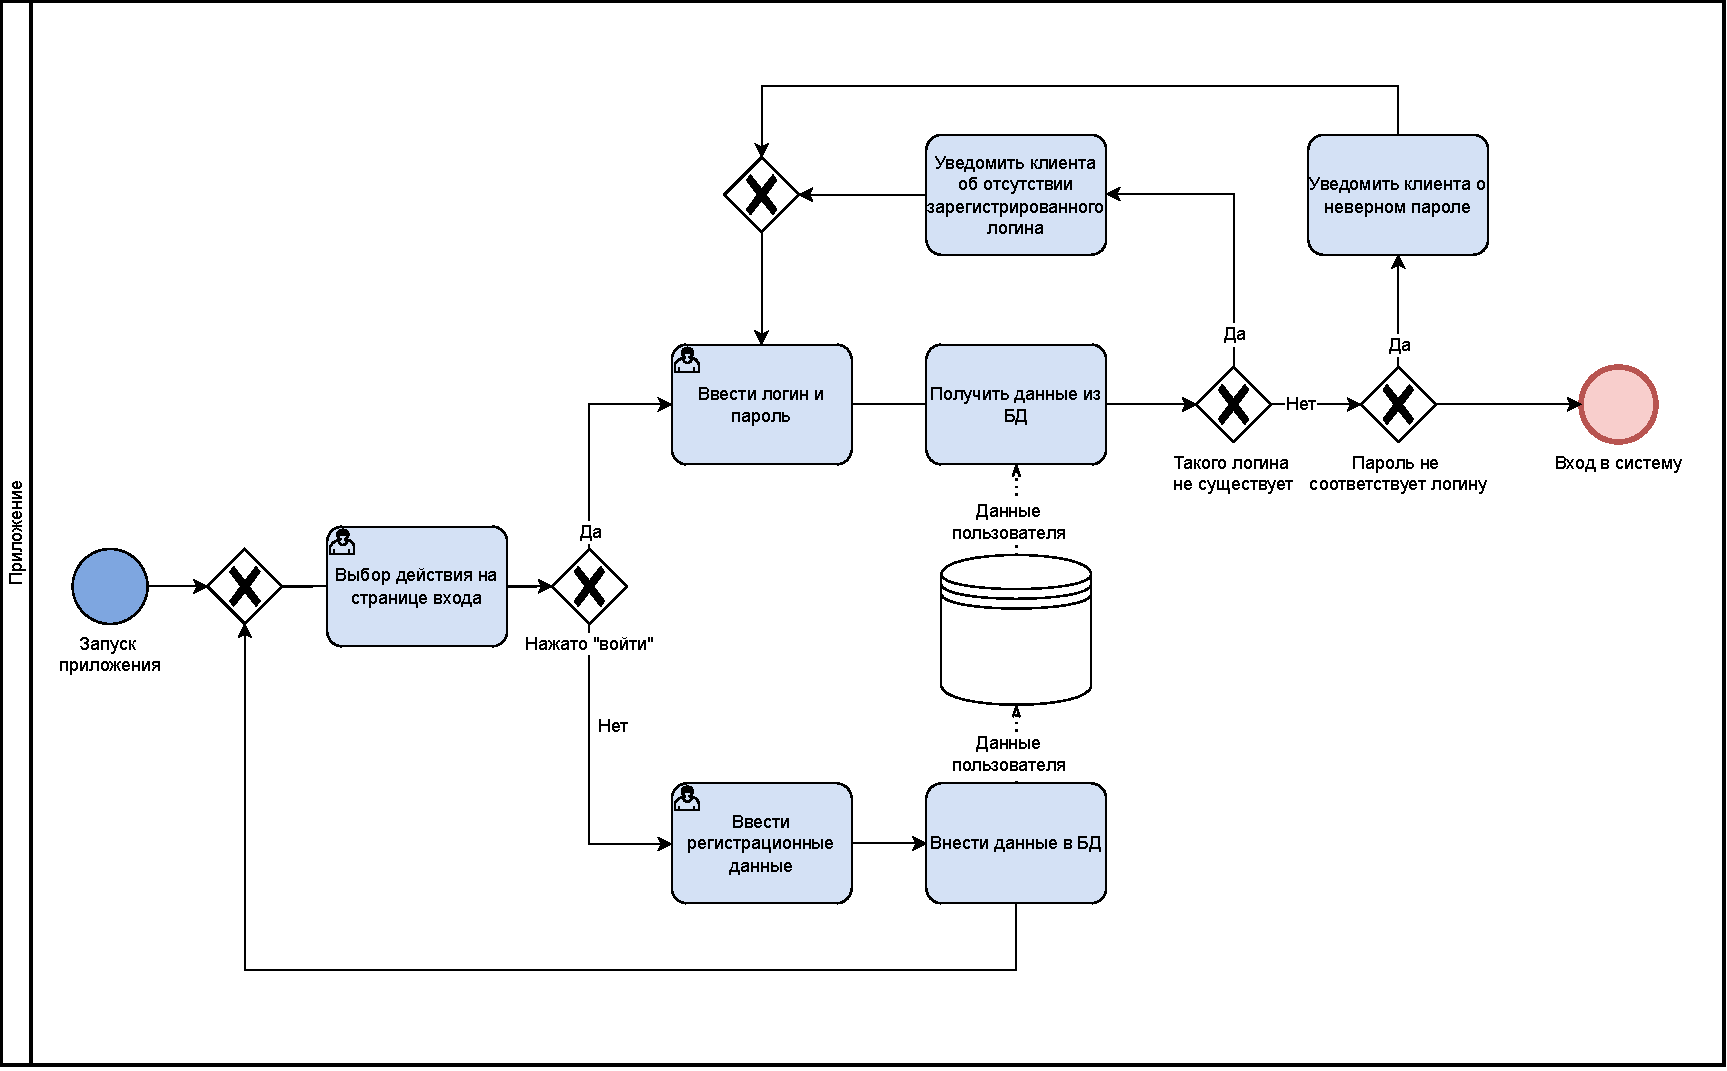
\includegraphics[width=0.9\linewidth]{assets/images/BPMN-Авторизация.pdf}
	\caption{Бизнес-процесс авторизации и регистрации пользователей}
	\label{fig:BPMN-auth}
\end{figure}

Формализация бизнес-процесса создания новых событий с возможностью приглашения к ним участников представлена на рисунке \ref{fig:BPMN-event}.

\begin{figure}[ht!]
	\centering
	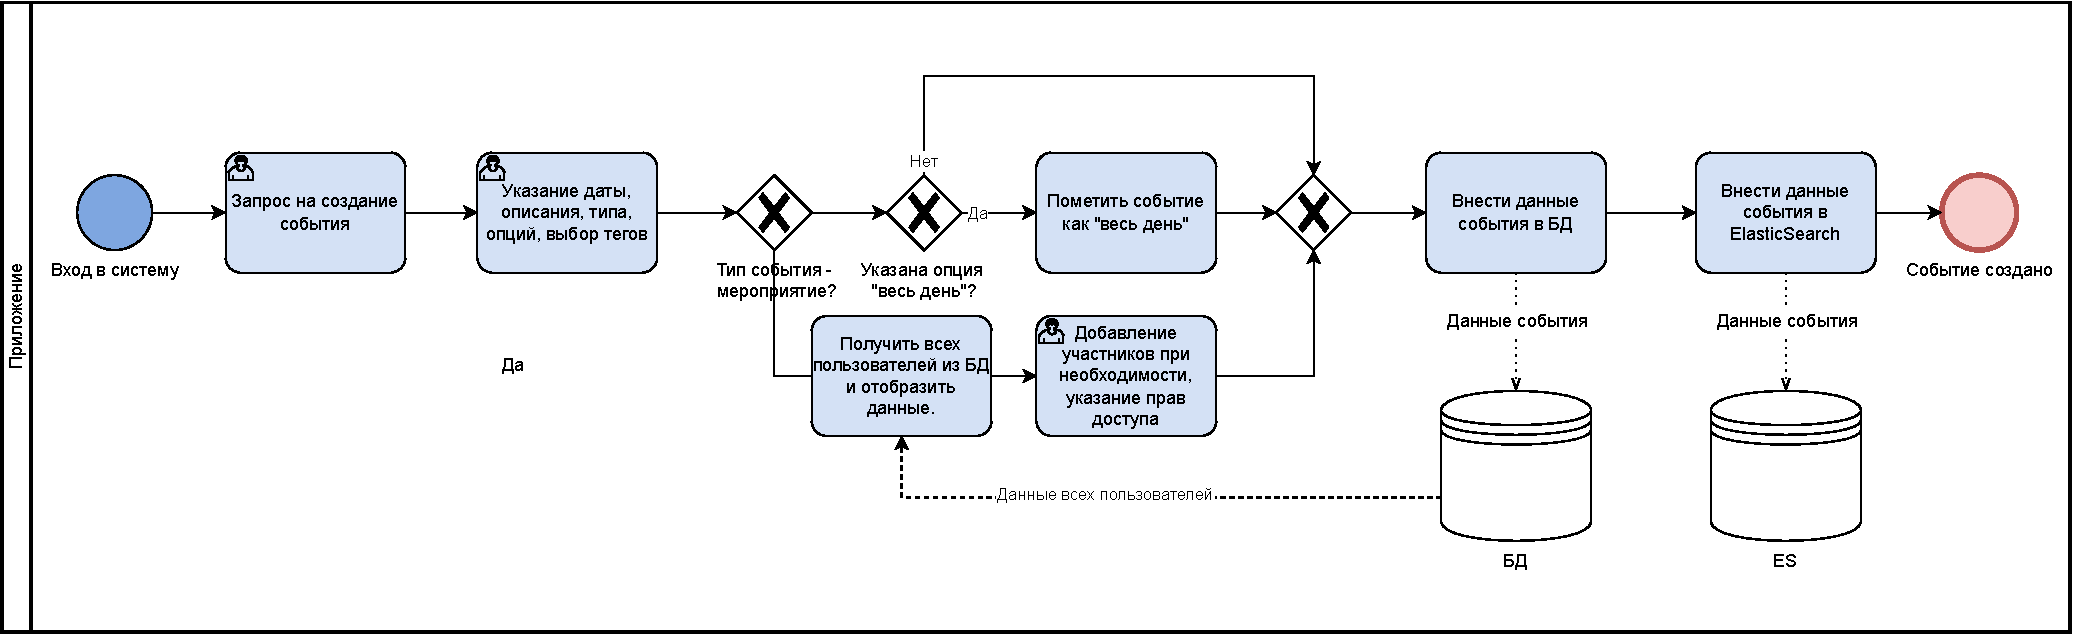
\includegraphics[width=1\linewidth]{assets/images/BPMN-Создание-события.pdf}
	\caption{Бизнес-процесс авторизации и регистрации пользователей}
	\label{fig:BPMN-event}
\end{figure}
